\chapter{Теоретическая часть}
\label{cha:theory}

\section{Определения}

\textbf{Корпус} --- множество подобранных и определённым образом обработанных текстов.

\textbf{Токен} --- элементарная единица разбиения корпуса.

\textbf{Токенизация} --- процесс разбиения корпуса на токены с присвоением им уникальных числовых идентификаторов.

\textbf{Языковая модель} --- распределение $P(w_t | w_1,w_2,w_3,\dots,w_n)$ вероятностей встретить токен $w_t$ в корпусе сразу после $n$ токенов $w_i$, $i\in[1, n]$, идущих подряд, где $w_i \in W \, \forall i$, $W$ --- множество всех токенов корпуса, $n$ --- длина контекста модели.

\textbf{Длина контекста} --- количество $n$ токенов $w_i$, $i\in[0, n]$, предшествующих токену $w_t$, от которых зависит вероятность появления в тексте токена $w_t$.

\textbf{Дообучение} --- процесс обучения уже обученной на некоторых данных модели машинного обучения на новых данных. В случае языковой модели это означает подстройку модели под новое распределение токенов.

\textbf{Перплексия} --- мера схожести двух вероятностных распределений, используемая для оценки качества генерации текста языковой моделью. Перплексия задаётся формулой \ref*{eq:perplexity}.
\begin{equation}
    \label{eq:perplexity}
    \textrm{PP}(W)=\sqrt[n]{\frac{1}{P(w_1,w_2,\dots,w_n)}}
\end{equation}

\section{Постановка задачи}

Дано:
\begin{enumerate}
    \item корпус, состоящий из текстов, принадлежащих конкретной предметной области;
    \item предобученная нейросетевая языковая модель, хорошо моделирующая вероятностное распределение слов в естественном языке.
\end{enumerate}
Требуется:
\begin{enumerate}
    \item дообучить данную языковую модель на данных из корпуса, получив новую языковую модель, моделирующую распределение вероятностей слов в данном корпусе;
    \item реализовать возможность применения её для генерации новых текстов, принадлежащих предметной области данного корпуса;
    \item создать графический интерфейс для взаимодействия пользователя с моделью;
    \item подготовить получившееся приложение для дистрибуции.
\end{enumerate}

\section{Нейронные сети}

\subsection{Однослойный перцептрон}

Одной из простейших моделей машинного обучения является однослойный перцептрон. Он позволяет, обучаясь на выборке данных, решать задачу линейной регрессии, то есть, устанавливать зависимость между зависимой переменной $y$ и независимыми переменными $x$ при условии, что между ними существует линейная зависимость, которую можно описать уравнением \ref*{eq:lin_reg}. В нём всегда $x_0\equiv 1$, а $w_0$ называется смещением, так как изменение этой компоненты приводит к увеличению или уменьшению $y$ на постоянное значение.
\begin{equation}
    \label{eq:lin_reg}
    y=\mathbf{w}\cdot\mathbf{x}=w_0x_0+w_1x_1+w_2x_2+\dots+w_nx_n,\quad x_0\equiv 1
\end{equation}

В этом уравнении неизвестными являются компоненты вектора $\mathbf{w}$, найдя которые, можно получить взаимосвязь между $x$ и $y$. Обучающая выборка данных представляет собой матрицу $\mathbf{X}$ размера $m \times (n+1)$ наблюдений вектора $\mathbf{x}$ и вектор $\mathbf{y}$ размера $m$, где $y_i=\mathbf{w} \cdot \mathbf{x}_i$, $\mathbf{x}_i$ --- $i$-я строка матрицы $\mathbf{X}$, как показано в уравнении \ref*{eq:lin_reg_dataset}.
\begin{equation}
    \label{eq:lin_reg_dataset}
    \mathbf{X}\mathbf{w}=
    \left(\begin{matrix}
        x_0^1 & x_1^1 & x_2^1 & x_3^1 & \dots & x_n^1 \\
        x_0^2 & x_1^2 & x_2^2 & x_3^2 & \dots & x_n^2 \\
        x_0^3 & x_1^3 & x_2^3 & x_3^3 & \dots & x_n^3 \\
        x_0^4 & x_1^4 & x_2^4 & x_3^4 & \dots & x_n^4 \\
        \vdots & \vdots & \vdots & \vdots & \ddots & \vdots \\
        x_0^m & x_1^m & x_2^m & x_3^m & \dots & x_n^m
    \end{matrix}\right)
    \left(\begin{matrix}
        w_0 \\
        w_1 \\
        w_2 \\
        \vdots \\
        w_n
    \end{matrix}\right)=
    \left(\begin{matrix}
        y_1 \\
        y_2 \\
        y_3 \\
        y_4 \\
        \vdots \\
        y_m
    \end{matrix}\right)=\mathbf{y}
\end{equation}

Уравнение \ref*{eq:lin_reg_dataset} имеет одно решение относительно $\mathbf{w}$ тогда и только тогда, когда $\rank \mathbf{X} = n$. Если $\rank \mathbf{X} < n$, уравнение имеет бесконечное число решений, и если $\rank \mathbf{X} > n$, уравнение не имеет решений. Но на практике данных обычно больше, чем компонент в векторе $\mathbf{w}$, поэтому используется аппроксимация методом наименьших квадратов, суть которой состоит в том, чтобы путём решения задачи минимизации, показанной в уравнении \ref*{eq:lsm}, найти такую прямую, чтобы функция потерь $L(\mathbf{y},\hat{\mathbf{y}})$ была минимальна.
\begin{equation}
    \label{eq:lsm}
    \begin{cases}
        \mathbf{w} = \arg\min\limits_\mathbf{w} L(\mathbf{y},\hat{\mathbf{y}}), \\
        \hat{\mathbf{y}}=\mathbf{X}\mathbf{w}
    \end{cases}
\end{equation}

Из курса математической статистики известно, что лучше всего в данной задаче подходит функция потерь $\MSE$ или средний квадрат ошибки (формула \ref*{eq:mse}). При использовании этой функции потерь дисперсия ошибки получается наименьшей.
\begin{equation}
    \label{eq:mse}
    \MSE(\mathbf{y},\hat{\mathbf{y}})=\sum\limits_{i=1}^m(\mathbf{x}_i^\mathsf{T}\mathbf{w}-y_i)^2=(\mathbf{X}\mathbf{w}-\mathbf{y})^\mathsf{T}(\mathbf{X}\mathbf{w}-\mathbf{y})
\end{equation}

Минимум функции потерь можно найти градиентными методами, например, методом Adam, так как она дифференцируема, и её производную можно вычислить аналитически (формула \ref*{eq:mse_der}). Процесс поиска минимума функции потерь модели называют обучением.
\begin{equation}
    \label{eq:mse_der}
    \frac{\partial\MSE}{\partial \mathbf{w}}(\mathbf{w})=2\mathbf{X}^\mathsf{T}(\mathbf{X}\mathbf{w}-\mathbf{y})
\end{equation}

Если же от модели требуется предсказывать не численные характеристики объектов, а относить их к той или иной группе, то такая задача называется задачей классификации, а модель --- логистической регрессией.

В этом случае требуется не аппроксимировать точки гиперплоскостью, а сделать так, чтобы гиперплоскость отделяла точки одного класса от точек другого (рисунок \ref*{fig:log_reg}). Для этого к выходу линейной регрессии дополнительно применяют функцию с областью значений $[0, 1]$, чтобы выход модели можно было интерпретировать как вероятность принадлежности объекта заданному классу \cite{art:linear_models}.
\begin{figure}[h]
    \centering
    \includegraphics[width=0.5\textwidth]{../inc/images/logistic_regression.png}
    \caption{Работа логистической регрессии в случае бинарной классификации}
    \label{fig:log_reg}
\end{figure}

\begin{equation}
    \label{eq:sigmoid}
    \sigma(x)=\frac{1}{1+e^{-x}}
\end{equation}

\begin{figure}[h]
    \centering
    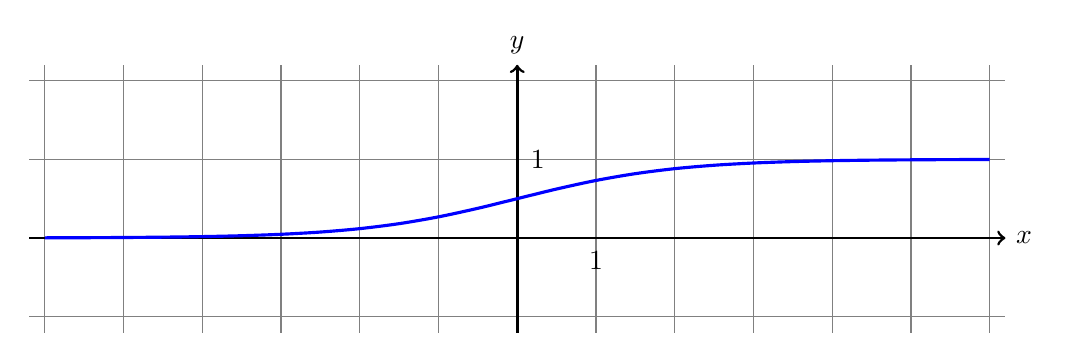
\begin{tikzpicture}[domain=-6:6]
        \draw[thin,color=gray] (-6.2,-1.2) grid (6.2,2.2);
      
        \draw[line width=0.35mm,->] (-6.2,0) -- (6.2,0) node[right] {$x$};
        \draw[line width=0.35mm,->] (0,-1.2) -- (0,2.2) node[above] {$y$};

        \draw[line width=0.4mm,color=blue,smooth] plot (\x,{1/(1+exp(-\x))});

        \draw[] (0.05, 1) node[right] {$1$};
        \draw[] (1, -0.05) node[below] {$1$};
    \end{tikzpicture}
    \caption{График сигмоиды}
    \label{fig:sigmoid}
\end{figure}

\begin{equation}
    \label{eq:softmax}
    \Softmax(\mathbf{x})=\frac{1}{\sum\limits_{i=1}^n e^{x_i}}
    \left(\begin{matrix}
        e^{x_1} \\
        e^{x_2} \\
        e^{x_3} \\
        \vdots \\
        e^{x_n}
    \end{matrix}\right),\quad \mathbf{x}\in \R^n
\end{equation}

В случае бинарной классификации, то есть, когда класса два, в роли такой функции выступает сигмоида (формула \ref*{eq:sigmoid}, рисунок \ref*{fig:sigmoid}). Тогда выход модели трактуется как вероятность принадлежности объекта первому классу. Если же классов больше двух, то на выходе модели должен получиться вектор, содержащий столько компонент, сколько в задаче классов, и к нему применяется функция $\Softmax$ (формула \ref*{eq:softmax}), выход которой удовлетворяет аксиомам вероятности \ref*{eq:prob_axioms}.
\begin{equation}
    \label{eq:prob_axioms}
    \begin{cases}
        \mathbf{y}=\left(\begin{matrix}
            y_1 & y_2 & y_3 & \dots & y_n
        \end{matrix}\right)^\mathsf{T} \\
        y_i \in [0, 1]\,\forall i\in[1, n], \\
        \sum\limits_{i=1}^n y_i = 1
    \end{cases}
\end{equation}

В задаче классификации используется функция потерь, называемая перекрёстной энтропией (формула \ref*{eq:ce_loss}). В случае бинарной классификации она представляется в виде \ref*{eq:bce_loss}.
\begin{equation}
    \label{eq:ce_loss}
    \CE(\mathbf{y},\hat{\mathbf{y}})=-\sum\limits_{i=1}^n y_i \ln \hat{y}_i
\end{equation}
\begin{equation}
    \label{eq:bce_loss}
    \BCE(y,\hat{y})=-y \ln \hat{y} - (1-y)\ln (1-\hat{y})
\end{equation}

\subsection{Нелинейная аппроксимация}

Модели линейной и логистической регрессии позволяют строить аппроксимации только гиперплоскостями. Чтобы иметь возможность аппроксимировать нелинейные зависимости в данных, их применяют последовательно, перемежая нелинейными функциями, например, как в формуле \ref*{eq:nn_sample}. Тогда функция $f(x)$ называется нейронной сетью, а линейные модели, из которых она состоит --- её слоями. Параметры, или веса, нейронной сети, состоят из параметров всех её слоёв, а оптимизируются они так же, градиентными методами.
\begin{equation}
    \label{eq:nn_sample}
    f(x)=\sigma(\dots \sigma(\sigma(xw_1)w_2)w_3 \dots)
\end{equation}

Функции, перемежающие применения линейных слоёв, называются функциями активации. Они могут быть любыми кусочно-гладкими нелинейными функциями, а на то, какие операции производятся над слоями внутри нейронной сети, накладывается только одно ограничение: функция $f(x)$ должна оставаться кусочно-гладкой, чтобы можно было искать минимум функции потерь градиентными методами.

\section{Градиентные методы оптимизации}

Минимум функции потерь при обучении нейронных сетей обычно ищется градиентными методами, которые хорошо себя зарекомендовали в решении задач на оптимизацию дифференцируемых функций.

Суть этой группы методов хорошо иллюстрировать на примере простейшего из них --- градиентного спуска.

Пусть имеется задача, представленная в виде системы \ref*{eq:grad_desc_problem}.
\begin{equation}
    \label{eq:grad_desc_problem}
    \begin{cases}
        L(\mathbf{w}): \R^n \rightarrow \R, \\
        \nabla L(\mathbf{w}) = \left(\begin{matrix}
            \frac{\partial L}{\partial w_1}(w_1) &
            \frac{\partial L}{\partial w_2}(w_2) &
            \frac{\partial L}{\partial w_3}(w_3) &
            \hdots &
            \frac{\partial L}{\partial w_n}(w_n)
        \end{matrix}\right)^\mathsf{T}, \\
        L(\mathbf{w}) \rightarrow \min\limits_\mathbf{w}
    \end{cases}
\end{equation}

Требуется найти минимум дифференцируемой функции $n$ переменных. Как известно из курса математического анализа, градиент функции нескольких переменных, вычисленный в конкретной точке --- это вектор, указывающий направление наискорейшего возрастания функции в этой точке. Значит, чтобы найти минимум, двигаясь из какой-либо начальной точки, нужно перемещаться в направлении, противоположном градиенту. Эту идею реализует градиентный спуск (формула \ref*{eq:grad_desc_algo}).
\begin{equation}
    \label{eq:grad_desc_algo}
    \mathbf{w}^{t+1}=\mathbf{w}^t-\alpha\nabla L(\mathbf{w})
\end{equation}

Делая шаги длины $\alpha$ в направлении антиградиента функции, с увеличением $t$ алгоритм приближается к минимуму.

Но у этого алгоритма есть ряд проблем, связанных со скроростью сходимости. Наглядный пример приведён на рисунке \ref*{fig:grad_desc_problem}. В нём целевая функция представляет собой вытянутый параболоид, и градиентный спуск в этом случае делает шаги неоптимальным образом, двигаясь к точке минимума очень медленно.

\begin{figure}[h]
    \centering
    \includegraphics[width=0.5\textwidth]{../inc/images/gradient_descend_problem.png}
    \caption{Проблема долгой сходимости простого градиентного спуска}
    \label{fig:grad_desc_problem}
\end{figure}

Одним из решений этой проблемы является введение физических характеристик для точки, двигающейся по поверхности целевой функции. Например, в методе Adam (англ. --- Adaptive Moment Estimation) вводятся масса и скорость, моделируя движение шарика вниз по неровной поверхности.

Другая проблема состоит в том, что фиксированный шаг градиентного спуска может мешать оптимизации функции по некоторым координатам. В методе Adam это решается путём введения специальных весов, уменьшающих шаг по координатам, которые часто изменяются. Метод Adam описывается формулами \ref*{eq:adam}.
\begin{equation}
    \label{eq:adam}
    \begin{cases}
        \mathbf{m}^t=\beta_1\mathbf{m}^{t-1}+(1-\beta_1)\nabla L(\mathbf{w}) \\
        \mathbf{v}^t=\beta_2\mathbf{v}^{t-1}+(1-\beta_2)(\nabla L(\mathbf{w}))^2 \\
        \hat{\mathbf{m}}^t=\frac{\mathbf{m}^t}{1-\beta_1^t} \\
        \hat{\mathbf{v}}^t=\frac{\mathbf{v}^t}{1-\beta_2^t} \\
        \mathbf{w}^{t+1}=\mathbf{w}^t-\frac{\alpha}{\sqrt{\hat{\mathbf{v}}^t}+\varepsilon}\hat{\mathbf{m}}^t \\
        \mathbf{m}^0=\mathbf{0},\quad\mathbf{v}^0=\mathbf{0}
    \end{cases}
\end{equation}

Параметры $\beta_1$, $\beta_2$, $\varepsilon$ и $\alpha$ задаются по усмотрению пользователя в зависимости от решаемой задачи.

На сегодняшний день Adam является одним из лучших алгоритмов оптимизации, показывающих наименьшее время сходимости при обучении нейронных сетей на разнообразных данных \cite{art:optimizers}.

\section{Стохастический градиентный спуск}

На практике бывает так, что данных настолько много, что одновременно они не помещаются в оперативную память компьютера или видеокарты, из-за чего становится невозможно вычислить градиент функции потерь на всей обучающей выборке. Поэтому обычно применяется стохастический градиентный спуск, смысл которого сводится к рассчёту функции потерь при использовании подвыборки обучающих данных.

Пусть $\mathbf{X}$ --- обучающая выборка данных, содержащая $n$ наблюдений. Она разбивается на $m$ подвыборок одинакового размера, и функция потерь считается на каждой из них независимо, как в формуле \ref*{eq:sgd}.

\begin{equation}
    \label{eq:sgd}
    \mathbf{w}^{t+1}=\mathbf{w}^t-\alpha \nabla L_i(\mathbf{w}^t)
\end{equation}

Здесь $L_i(\mathbf{w}^t)$ --- функция потерь, посчитанная на $i$-й подвыборке $\mathbf{x}_i$. Важно, что при всех $i\in[1, m]$ $L_i(\mathbf{w}^t)$ считается в одной и той же точке $\mathbf{w}^t$. После завершения итераций по $i$ подвыбоки случайным образом перемешиваются, и расчёт повторяется в новой точке $\mathbf{w}^{t+1}$.

\section{Токенизация}

Одним из важнейших понятий области обработки естественного языка является токенизация. Так как нейронные сети работают с векторами, то есть, с числами, для решения с их помощью задачи обработки текста требуется эти тексты представлять в виде векторов.

Суть токенизации сводится к дроблению текста на токены, некие элементарные единицы, с последующей их заменой на числа, соответствующие их номерам в списке уникальных токенов текста. Такой подход позволяет однозначно отображать тексты в вектора, которые можно обрабатывать нейронными сетями, а также, наоборот, декодировать текст из векторов.

Токенизация бывает основана на словах, частях слов и символах. У каждого из её видов есть свои преимущества и недостатки.

Так, если брать за токены слова, то теряется информация о словообразовании и словоформах, даже одно слово в разных падежах будет для модели двумя совершенно разными токенами. Зато, если обрезать у слов окончания, то токены будут совпадать, и на таких данных уже можно обучить простую модель, решающую, например, задачу классификации текстов. Но, конечно, такой способ кодирования не подходит для генерации текста ввиду потери важной информации об окончаниях.

Если за токены брать отдельные символы текста, то в теории вся исходная информация из текста сохранится. Но на практике эта информация будет слишком разрежена, и для её использования понадобится слишком сложная модель и огромное количество данных.

В естественном, например, русском языке элементарными единицами словообразования являются морфемы, которые состоят из больше чем одного символа, и разделение текста на них сохранит всю информацию о возможных вариациях слов, которая при этом будет не слишком разреженной. Таким образом, для моделирования языка лучше всего подходит токенизация, берущая за основу части слов.

Но алгоритм деления слов на морфемы очень сложен и узко специализирован для работы с конкретным языком. А в обучающей выборке могут встретиться тексты на разных языках, и нужно, чтобы модель могла их все обработать. Для решения этой задачи существует алгоритм BPE (англ. --- Byte-Pair Encoding), изначально разработанный для сжатия данных.

Суть его состоит в том, что для всех пар символов из обучающей выборки считается частота, с которой они встречаются вместе. Затем самые частотные пары остаются в виде самостоятельных токенов, токены с нулевой частотой отбрасываются, а остальные остаются как есть. Далее процесс повторяется до тех пор, пока не останется возможности объединять токены в пары или пока не будет превышено максимальное число итераций.

Для больших корпусов алгоритм BPE позволяет создать оптимальный словарь токенов при минимальном их числе \cite{art:bpe}.

\section{Языковые модели}

Задача генерации текста на естественном языке сводится к задаче моделирования языка. Языковая модель --- это условное распределение вероятности встретить в тексте токен $w_{n+1}$ сразу после $n$ токенов $\{w_i\}_{i=1}^n$, где $n$ --- длина контекста модели, то есть, максимально возможное количество токенов, влияющих на появление токена $w_{n+1}$.

Нейросетевые языковые модели принимают на вход вектор длины $n$, содержащий токены контекста, и выдают вектор длины, равной количеству токенов в словаре, к которому применяется функция $\Softmax$, чтобы получить вектор, в котором каждому токену сопоставлена вероятность, что он идёт после заданных $n$ токенов контекста. Такая модель схематично изображена на рисунке \ref*{fig:lang_model} \cite{art:lang_models}.

\begin{figure}[h]
    \centering
    \includegraphics[width=0.8\textwidth]{../inc/images/language_model.png}
    \caption{Простая нейросетевая языковая модель}
    \label{fig:lang_model}
\end{figure}

Как видно, задача языкового моделирования является частным случаем задачи многоклассовой классификации. Поэтому, при обучении в качестве функции потерь используется перекрёстная энтропия.

Для того, чтобы решить задачу генерации текста с помощью языковой модели, нужно просто генерировать случайные числа из распределения, получаемого на выходе функции $\Softmax$, с проведением обратного преобразования токенов в текст, добавлять новый токен в конец вектора контекста с удалением первого и генерацией нового токена до тех пор, пока не будет сгенерирован текст желаемой длины.

\section{Рекуррентные нейронные сети}

Так как текст представляет собой последовательность токенов, а определение языковой модели подразумевает зависимость вероятности следующих токенов от нескольких предыдущих, естественно попробовать реализовать алгоритм его обработки, который бы учитывал эту рекуррентность.

Примером таких моделей являются рекуррентные нейронные сети (англ. --- Recurrent Neural Networks, RNN). Их особенность состоит в наличии так называемого скрытого состояния --- вектора, накапливающего в себе информацию, полученную от поэлементной обработки входной последовательности, как отражено в формулах \ref*{eq:rnn_hidden_state}. Здесь $x_t$ --- вход слоя, $w_{hh}$, $w_{xh}$, $w_{hy}$ --- обучаемые параметры слоёв сети, $y_t$ --- выход слоя, $h_t$ --- скрытое состояние на шаге $t$, $\Th(\cdot)$ --- гиперболический тангенс (формула \ref*{eq:tanh}, рисунок \ref*{fig:tanh}).

\begin{equation}
    \label{eq:rnn_hidden_state}
    \begin{cases}
        h_t = \Th(w_{hh}h_{t-1}+w_{xh}x_t) \\
        y_t = w_{hy}h_t
    \end{cases}
\end{equation}

\begin{equation}
    \label{eq:tanh}
    \Th(x)=\frac{e^x-e^{-x}}{e^x+e^{-x}}
\end{equation}

Схематическое изображение RNN представлено на рисунке \ref*{fig:rnn}.

\begin{figure}[H]
    \centering
    \includegraphics[width=0.8\textwidth]{../inc/images/rnn.png}
    \caption{Схема работы рекуррентной нейронной сети}
    \label{fig:rnn}
\end{figure}

\begin{figure}[H]
    \centering
    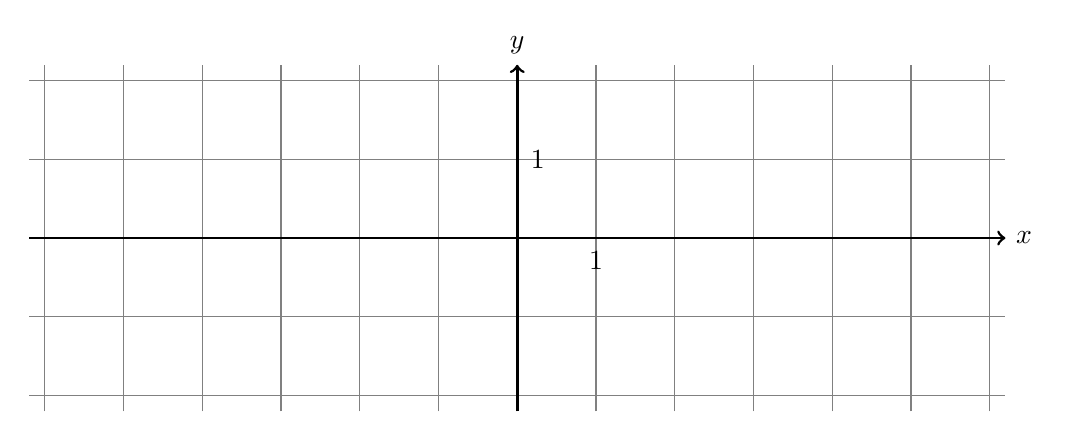
\begin{tikzpicture}[domain=-6:6]
        \draw[thin,color=gray] (-6.2,-2.2) grid (6.2,2.2);
      
        \draw[line width=0.35mm,->] (-6.2,0) -- (6.2,0) node[right] {$x$};
        \draw[line width=0.35mm,->] (0,-2.2) -- (0,2.2) node[above] {$y$};

        \draw[line width=0.4mm,color=blue,smooth] plot function{(exp(x)-exp(-x))/((exp(x)+exp(-x)))};

        \draw[] (0.05, 1) node[right] {$1$};
        \draw[] (1, -0.05) node[below] {$1$};
    \end{tikzpicture}
    \caption{График гиперболического тангенса}
    \label{fig:tanh}
\end{figure}

\begin{figure}[H]
    \centering
    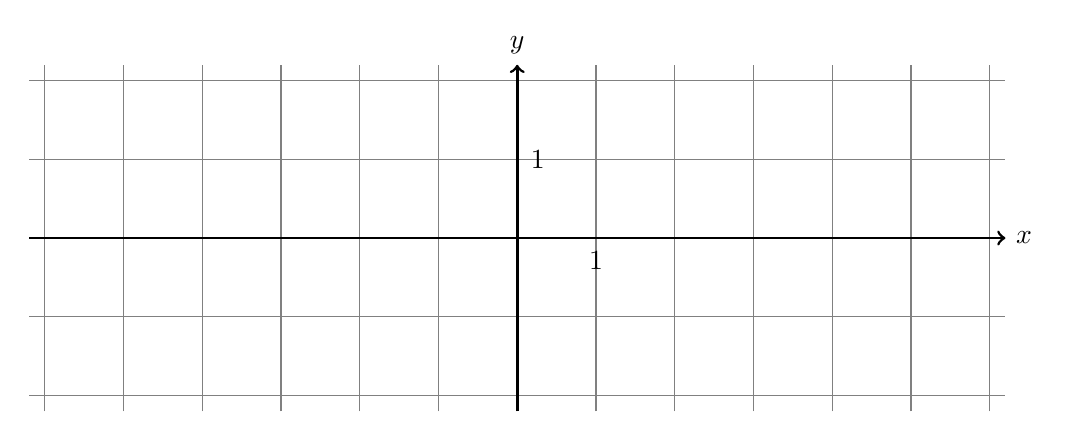
\begin{tikzpicture}[domain=-6:6]
        \draw[thin,color=gray] (-6.2,-2.2) grid (6.2,2.2);
      
        \draw[line width=0.35mm,->] (-6.2,0) -- (6.2,0) node[right] {$x$};
        \draw[line width=0.35mm,->] (0,-2.2) -- (0,2.2) node[above] {$y$};

        \draw[line width=0.4mm,color=blue,smooth] plot function{1-((exp(x)-exp(-x))/((exp(x)+exp(-x))))*((exp(x)-exp(-x))/((exp(x)+exp(-x))))};

        \draw[] (0.05, 1) node[right] {$1$};
        \draw[] (1, -0.05) node[below] {$1$};
    \end{tikzpicture}
    \caption{График производной гиперболического тангенса}
    \label{fig:tanh_der}
\end{figure}

Рекуррентные нейронные сети способны улавливать зависимости в последовательных данных, но у них есть недостатки. Как видно на рисунке \ref*{fig:tanh_der}, производная гиперболического тангенса, используемого в качестве функции активации в RNN, почти на всей области определения близка к нулю. На практике это означает, что чем длиннее последовательность данных, тем больше в формуле производной функции потерь будет множителей, близких к нулю, и тем ближе к нулю будут шаги градиентного спуска, что замедляет обучение, а иногда делает его и вовсе невозможным. С этим связана вторая проблема --- новые данные в последовательности оказывают на результат большее влияние, чем старые за счёт многократного умножения последних на близкие к нулю числа. Иными словами можно сказать, что нейросеть <<забывает>> старые данные.

\section{Модификации RNN}

Для решения этой проблемы существуют две основные модификации RNN, общая идея которых сводится к введению дополнительных блоков для предсказания степени важности пришедших на вход данных, обеспечивая более контролируемое забывание.

\subsection{GRU}

Архитектура GRU (англ. --- Gated Recurrent Unit) предлагает решать проблему забывания с помощью ряда так называемых вентилей:
\begin{itemize}
    \item вентиль обновления, определяющий количество информации, которое требуется сохранить с предыдущей итерации (формула \ref*{eq:gru_update});
    \item вентиль забывания, определяющий количество информации, которое требуется забыть (формула \ref*{eq:gru_reset}).
\end{itemize}

\begin{equation}
    \label{eq:gru_update}
    z_t = \sigma(w_{zx}x_t+w_{zh}h_{t-1})
\end{equation}

\begin{equation}
    \label{eq:gru_reset}
    r_t = \sigma(w_{rx}x_t+w_{rh}h_{t-1})
\end{equation}

Информация, которую будет хранить текущая ячейка сети, рассчитывается по формуле \ref*{eq:gru_current}, а итоговое значение скрытого состояния --- по формуле \ref*{eq:gru_state}.

\begin{equation}
    \label{eq:gru_current}
    c_t = \Th(w_{cx}x_t+w_{ch}r_th_{t-1})
\end{equation}

\begin{equation}
    \label{eq:gru_state}
    h_t = (1-z_t)h_{t-1}+z_tc_t
\end{equation}

Здесь $\sigma(\cdot)$ --- сигмоида, а $w_{zx}$, $w_{zh}$, $w_{rx}$, $w_{rh}$, $w_{cx}$, $w_{ch}$ --- обучаемые параметры слоя.
Схема ячейки GRU изображена на рисунке \ref*{fig:gru}.

\begin{figure}[h]
    \centering
    \includegraphics[width=0.5\textwidth]{../inc/images/gru.png}
    \caption{Схема ячейки GRU}
    \label{fig:gru}
\end{figure}

\subsection{LSTM}

Нейронная сеть с долгой краткосрочной памятью (англ. --- Long Short-Term Memory, LSTM) предлагает решение для борьбы с забыванием, благодаря которому сети удаётся сохранять в 4 раза больше информации, чем обычной RNN \cite{art:rnn}.

Эта архитектура тоже оперирует понятием вентиля, их в ней три:
\begin{itemize}
    \item входной вентиль, контролирующий поток приходящей информации (формула \ref*{eq:lstm_input});
    \item вентиль забывания, управляющий количеством информации, которое требуется сохранить с предыдущей итерации (формула \ref*{eq:lstm_forget});
    \item выходной вентиль, контролирующий поток выходящей информации (формула \ref*{eq:lstm_output}).
\end{itemize}

\begin{equation}
    \label{eq:lstm_input}
    i_t = \sigma(w_{ix}x_t+w_{ih}h_{t-1})
\end{equation}

\begin{equation}
    \label{eq:lstm_forget}
    f_t = \sigma(w_{fx}x_t+w_{fh}h_{t-1})
\end{equation}

\begin{equation}
    \label{eq:lstm_output}
    o_t = \sigma(w_{ox}x_t+w_{oh}h_{t-1})
\end{equation}

Далее вычисляются промежуточные значения $g_t$ и $s_t$ (формулы \ref*{eq:lstm_input_node} и \ref*{eq:lstm_hidden}), а с их помощью считается результирующее скрытое состояние $h_t$ по формуле \ref*{eq:lstm_state}.

\begin{equation}
    \label{eq:lstm_input_node}
    g_t = \Th(w_{gx}x_t+w_{gh}h_{t-1})
\end{equation}

\begin{equation}
    \label{eq:lstm_hidden}
    s_t = s_{t-1}f_t+g_ti_t
\end{equation}

\begin{equation}
    \label{eq:lstm_state}
    h_t = \Th(s_t)o_t
\end{equation}

$w_{ix}$, $w_{ih}$, $w_{fx}$, $w_{fh}$, $w_{ox}$, $w_{oh}$, $w_{gx}$, $w_{gh}$ --- обучаемые параметры.

Схема ячейки LSTM изображена на рисунке \ref*{fig:lstm}.

\begin{figure}[h]
    \centering
    \includegraphics[width=0.8\textwidth]{../inc/images/lstm.png}
    \caption{Схема ячейки LSTM}
    \label{fig:lstm}
\end{figure}

LSTM позволяют частично решить проблему забывания, но за счёт большого числа обучаемых параметров они долго обучаются и занимают много места в памяти. Кроме того, остаётся нерешённой проблема затухающих градиентов.

\section{Механизм внимания}

В задачах преобразования одной последовательности в другую, например, в задаче машинного перевода или преобразования текста в речь, проблема затухающих градиентов может частично решаться с помощью механизма внимания (англ. --- Attention).

Его суть состоит в добавлении в сеть дополнительных параметров, отвечающих за взаимосвязь между отдельными ячейками RNN.

Рассмотрим нейронную сеть, изображённую на рисунке \ref*{fig:seq2seq}.

\begin{figure}[h]
    \centering
    \includegraphics[width=\textwidth]{../inc/images/seq2seq.png}
    \caption{Модель машинного перевода}
    \label{fig:seq2seq}
\end{figure}

Она состоит из двух рекуррентных сетей. Первая RNN принимает на вход предложение и токен за токеном накапливает информацию о нём, получая в скрытом состоянии последней ячейки вектор, кодирующий входное предложение. Вторая RNN принимает на вход этот вектор, а затем каждая её ячейка на основе своего скрытого состояния предсказывает токены слов на русском языке до тех пор, пока не будет предсказан токен конца предложения.

У этого подхода есть существенный недостаток: скрытое состояние последней ячейки первой RNN хранит больше информации о последнем слове предложения, чем об остальных, причём чем раньше слово стоит в предложении, тем меньше информации о нём будет сохранено в силу причин, описанных выше. Получается, что <<развернуть>> из этого вектора предложение, которое было бы правильным переводом, вряд ли удастся. Решение этой проблемы предлагает механизм внимания.

Рассмотрим рисунок \ref*{fig:attention}. В отлиличие от рисунка \ref*{fig:seq2seq}, здесь выход ячейки второй RNN зависит не только от скрытого состояния первой сети, но и от скрытого состояния всех остальных ячеек первой RNN с разными весами. Это и есть внимание: в процессе обучения такая архитектура позволяет выводить зависимости выходных данных от разных частей входных, как бы обращая внимание на разные слова входного предложения.

\begin{figure}[h]
    \centering
    \includegraphics[width=\textwidth]{../inc/images/attention.png}
    \caption{Внимание}
    \label{fig:attention}
\end{figure}

Благодаря тому, что каждая ячейка второй RNN зависит от каждой ячейки первой, информация о входных данных не зануляется, тем самым отчасти решается проблема затухающих градиентов.

\section{Архитектура Transformer}

Архитектура Transformer предлагает совершенно иной подход к нейрсетевой обработке текстовых данных. Её разработчики в своей статье \cite{art:transformer} показывают, что отказавшись от рекуррентных слоёв, можно получить гораздо лучшие результаты работы модели, а также заметно ускорить её обучение.

Вместо рекуррентных слоёв предлагается использовать механизм внутреннего внимания (англ. --- Self-Attention), близкий по сути к обычному вниманию, описанному выше, но с одним отличием: оба аргумента функции внимания принадлежат одной и той же последовательности. Получается, веса слоёв внутреннего внимания кодируют внутренние зависимости между токенами входной последовательности.

Слоёв внутреннего внимания используется сразу несколько --- это позволяет им выучивать разные зависимости, кодируя разного рода отношения между токенами.

В связи с отказом от рекуррентности Transformer не имеет возможности обрабатывать данные произвольной длины. Модели этой архитектуры принимают на вход заранее заданное число токенов --- последовательность длины контекста. С другой стороны, в них нет проблемы затухания градиентов, а информация обо всех токенах учитывается в равной мере, и благодаря этому все лучшие современные языковые модели построены на основе архитектуры Transformer.

В том случае, если входная последовательность токенов короче, чем контекст модели, её дополняют сначала специальными токенами, обозначающими отсутствие слова, которые представляются нулями.

Другой позитивный аспект использования множественных независимых слоёв внутреннего внимания --- это возможность обучать их параллельно на видеокартах, что было затруднено в случае с RNN, где результат каждой ячейки зависел от результата предыдущей.

Схема модели архитектуры Transformer представлена на рисунке \ref*{fig:transformer}.

\begin{figure}[h]
    \centering
    \includegraphics[width=\textwidth]{../inc/images/transformer.png}
    \caption{Transformer}
    \label{fig:transformer}
\end{figure}

Модель состоит из двух смысловых блоков --- кодировщик и декодировщик. Первый возвращает промежуточное векторное представление входной последовательности, а второй снова получает из него текст.

\section{BERT}

Архитектура Transformer позволяет строить очень большие модели, содержащие сотни миллионов вараметров, и обучать их на видеокартах, распараллеливая вычисления. Такие модели способны усваивать гораздо более глубокие закономерности в данных, чем могли RNN, и это можно использовать для построения векторного представления текста --- эмбеддингов (англ. --- Embedding), которые, в свою очередь, можно подать на вход модели классификации и классифицировать тексты.

Для решения этой задачи хорошо подходит первая часть модели Transformer --- кодировщик, возвращающий вектор чисел, который можно использовать в качестве эмбеддинга \cite{art:bert}.

Модель, за основу которой была взята эта идея, называется BERT (англ. --- Bidirectional Encoder Representations from Transformers). Её схема изображена на рисунке \ref*{fig:bert}.

\begin{figure}[H]
    \centering
    \includegraphics[width=\textwidth]{../inc/images/bert.png}
    \caption{BERT}
    \label{fig:bert}
\end{figure}

BERT обучается для решения сразу двух задач:
\begin{enumerate}
    \item определение по двум поданным на вход предложениям, с какой вероятностью одно идёт после другого в тексте;
    \item предсказание слов, стоящих на месте пропусков, отмеченных токеном [MASK].
\end{enumerate}

Такой процесс обучения позволяет BERT усваивать глубинные закономерности в устройстве языка и возвращать эмбеддинги, хорошо подходящие для классификации, то есть такие, что в их пространстве кластеры эмбеддингов эквивалентны группам текстов, имеющих общие признаки: тему, жанр, эмоциональную окраску и т. д.

\section{GPT}

Transformer хорошо подходит и для решения задачи генерации текста. Для этого была создана модель GPT (англ. --- Generative Pre-trained Transformer).

Если BERT представляет собой первую часть модели Transformer --- кодировщик, то GPT, наоборот, является второй частью, то есть, декодировщиком. Принимая на вход последовательность токенов, она их кодирует и предсказывает вероятности токенов, и чем какая-то из них выше, тем вероятнее, что соответствующий токен идёт сразу после заданной последовательности.

Здесь присутствует параллель с моделью BERT, которая тоже способна предсказывать токены на основании заданного контекста, но там используется информация как о тексте до предсказываемого токена, так и о тексте после. В GPT же учитывается только информация после, так как эта модель создавалась специально для решения задачи генерации текста, и такой подход в этом случае лучше, так как он делает модель авторегрессивной: генерируя один токен за раз, при каждой следующей генерации модель учитывает информацию с предыдущих шагов, что позволяет генерировать тексты любой длины, хоть и с ограниченным размером окна контекста.

Схема модели GPT изображена на рисунке \ref*{fig:gpt}.

\begin{figure}[H]
    \centering
    \includegraphics[width=0.7\textwidth]{../inc/images/gpt.png}
    \caption{GPT}
    \label{fig:gpt}
\end{figure}

\subsection{Маскированное внутреннее внимание}

В модели GPT, в отличие от описанной выше Transformer, используется модифицированная версия слоя внутреннего внимания: вместо того, чтобы маскировать токены токеном [MASK], как в BERT, слой маскированного внутреннего внимания (англ. --- Masked Self-Attention) использует маску, показанную в формуле \ref{eq:attn_mask}. Маска представляет собой вектор, состоящий из $k$ идущих подряд единиц, после которых идут нули.
\begin{equation}
    \label{eq:attn_mask}
    M=\left(\begin{matrix}
        m_1 = 1 & \hdots & 1 & 1 & \hdots & m_{k+1} = 0 & \hdots & 0 & 0
    \end{matrix}\right)^\textsf{T}
\end{equation}

Здесь $k$ --- номер обрабатываемого токена. Маска поэлементно умножается на вектор контекста, что исключает возможность срабатывания внимания между $k$-м токеном и токенами, идущими после него.

Процесс обучения GPT с поэтапной работой механизма маскированного внутреннего внимания проиллюстрирован на рисунке \ref*{fig:gpt_training}.

\begin{figure}[H]
    \centering
    \includegraphics[width=\textwidth]{../inc/images/gpt_training.png}
    \caption{Процесс обучения GPT}
    \label{fig:gpt_training}
\end{figure}

На нём слева изображён вектор контекста, а справа --- слово, которое нужно предсказать на каждом этапе.

\subsection{Развитие идей GPT}

Модель GPT продемонстрировала беспрецедентное качество генерации на момент своего выхода, а модели GPT-2 и GPT-3 показали, что улучшения результата можно добиться с использованием той же самой архитектуры за счёт увеличения размера контекста, числа блоков декодировщика и объёма обучающей выборки \cite{art:gpt3}.

Так, GPT-2 имеет длину контекста от 768 токенов в версии Small до 1600 в версии Extra Large и от 10 до 48 слоёв декодировщика соответственно.

GPT-3 же имеет уже 2048 токенов контекста и от 96 до 128 блоков декодировщика в зависимости от версии.

\subsection{Другие приложения GPT}

Оказалось, что модели GPT настолько хорошо моделируют язык, что их можно использовать для решения задач помимо генерации текста.

Например, GPT-3 способна без дополнительного дообучения давать ответы на некоторые вопросы, переводить текст с одного языка на другой, а также делать краткую выжимку из длинного текста (задача суммаризации), если подать ей на вход текст в определённой форме.

А если произвести дообучение, то модели GPT могут показывать очень хорошие результаты в этих задачах. Ниже изображены схемы дообучения GPT с примерами формата входных данных для решения задач машинного перевода (рисунок \ref*{fig:gpt_translation}) и суммаризации (рисунок \ref*{fig:gpt_summarization}). Видно, что достаточно ввести специальный токен, обозначающий функцию, которую требуется применить к тексту \cite{art:gpt3}.

\begin{figure}[h]
    \centering
    \includegraphics[width=\textwidth]{../inc/images/gpt-translation.png}
    \caption{Использование GPT для машинного перевода с английского на французский}
    \label{fig:gpt_translation}
\end{figure}

\begin{figure}[h]
    \centering
    \includegraphics[width=\textwidth]{../inc/images/gpt-summarization.png}
    \caption{Использование GPT для суммаризации}
    \label{fig:gpt_summarization}
\end{figure}
